% !TeX program = xelatex
% !BIB program = biber
\documentclass[light]{lutbeamer}

\usepackage{pgfpages}
\usepackage{ragged2e}
\usepackage{booktabs}
\usepackage{amssymb}
\usepackage{fontawesome5}
\usepackage{tikz}
\usepackage{pgfplots}
\pgfplotsset{compat=1.18}
\addbibresource{references.bib}
\newcommand{\andbadge}{%
  \tikz[baseline=-0.6ex]\node[
    draw=blue!70!black,
    fill=blue!10,
    rounded corners=2pt,
    inner xsep=4pt,
    inner ysep=1pt,
    text=blue!70!black,
    font=\scriptsize\bfseries
  ]{AND};%
}
\newcommand{\givenbadge}{%
  \tikz[baseline=-0.6ex]\node[
    draw=red!70!black,
    fill=red!10,
    rounded corners=2pt,
    inner xsep=4pt,
    inner ysep=1pt,
    text=red!70!black,
    font=\scriptsize\bfseries
  ]{GIVEN};%
}

% ===================================================================
% METADATA (DERS KİMLİK BİLGİLERİ)
% ===================================================================
\setdepartment{OSTİM TEKNİK ÜNİVERSİTESİ}
\institute[Yazılım Mühendisliği]{YAZILIM MÜHENDİSLİĞİ BÖLÜMÜ}
\author[Mühendislik Fakültesi]{\\
Prof.~Dr.~Yalçın ATA \\
Prof.~Dr.~Arif DEMİR \\
Dr.~Öğr.~Üyesi~Muhammed ELMNEFİ \\
Dr.~Öğr.~Üyesi~Haydar KILIÇ \\
Dr.~Öğr.~Üyesi~Emel GÜVEN \\
Dr.~Öğr.~Üyesi~Ufuk ASIL \\
Öğr.~Gör.~Sema ÇİFTÇİ
}
\title{MATH 204 -- Olasılık ve İstatistik}
\subtitle{Hafta 2: Koşullu Olasılık, Aksiyomlar ve Çarpım Kuralı}
\date{2025--2026 Bahar Dönemi}

% ===================================================================
% OTOMATİK İÇİNDEKİLER (SUNUM AKIŞI)
% ===================================================================
\setcounter{tocdepth}{2}

\AtBeginSection[]{
  \begin{frame}{Sunum Akışı}
    \scriptsize
    \begin{columns}[T]
      \begin{column}{0.48\textwidth}
        \tableofcontents[sections={1-3}, currentsection]
      \end{column}
      \begin{column}{0.48\textwidth}
        \tableofcontents[sections={4-10}, currentsection]
      \end{column}
    \end{columns}
  \end{frame}
}

\begin{document}

\setbeamertemplate{navigation symbols}{}

% ===================================================================
% KAPAK SLAYTLARI
% ===================================================================

% Görsel Tam Kapak (Logolu)
\begin{frame}<article:0>[plain,noframenumbering]
    \begin{tikzpicture}[remember picture,overlay]
        \node[anchor=center, at=(current page.center), inner sep=0pt] {
            \includegraphics[width=\paperwidth, height=\paperheight]{logos/background_figure.jpg}
        };
    \end{tikzpicture}
\end{frame}

% Resmi Başlık Sayfası
\maketitle{}

% GENEL İÇERİK HARİTASI
\begin{frame}{İçindekiler}
  \scriptsize
  \begin{columns}[T]
    \begin{column}{0.48\textwidth}
      \tableofcontents[sections={1-3}]
    \end{column}
    \begin{column}{0.48\textwidth}
      \tableofcontents[sections={4-10}]
    \end{column}
  \end{columns}
\end{frame}

% ===================================================================
% İÇERİK: HAFTA 2
% ===================================================================

\section{Koşullu Olasılığa Giriş}
\subsection{Motivasyon ve ``Kısıtlı Dünya'' Fikri}

\begin{frame}{Motivasyon: Bilgiyi Filtrelemek ve Güncellemek}
    \begin{columns}[T]
        \begin{column}{0.6\textwidth}
            \begin{block}{Yeni Bilgi = Yeni Dünya}
                Koşullu olasılık, elimize geçen yeni veriye göre inancımızı (olasılığı) güncelleme sanatıdır.
            \end{block}
            
            \begin{itemize}
                \item \textbf{Tıbbi Teşhis:} "Test pozitif" bilgisi gelince, hastalık olasılığı \%1'den \%80'e fırlar mı? (Yoksa \%10'da mı kalır?)
                \item \textbf{Spam Filtreleri:} E-postada "Bedava" kelimesi geçiyorsa, spam olma olasılığı koşullu olarak artar.
                \item \textbf{Bilgisayarlı Görü:} Bir görüntüde "göz" tespit edilirse, etrafında "yüz" olma olasılığı yükselir.
            \end{itemize}
        \end{column}
        \begin{column}{0.38\textwidth}
            \begin{center}
                \includegraphics[width=\textwidth]{figures/week2_motivation_icon.png}
                
                \vspace{0.3cm}
                \tiny \textit{Ayıklama: Gürültüden sinyale geçiş.}
            \end{center}
        \end{column}
    \end{columns}
\end{frame}

\begin{frame}{Neden Koşullama Yaparız?}
    \begin{block}{Motivasyon}
        Bazı uygulamalarda, ilgilendiğimiz olayların olasılık yapısını, \textbf{belirli kısıtlamalar altında} veya \textbf{yeni bir bilgi edindiğimizde} incelememiz gerekir.
    \end{block}

    \begin{itemize}[<+->]
        \item Genel popülasyonda diyabet görülme olasılığı yerine, ``35--50 yaş arası Asyalı kadınlar'' grubundaki olasılık daha anlamlı olabilir.
        \item Bir sistemin arızalanma olasılığı, ``sıcaklığın $100^\circ$C'yi geçtiği bilindiğinde'' değişecektir.
        \item \textbf{Ana Fikir:} Ek bilgi (additional information), belirsizliği azaltır ve örneklem uzayımızı daraltır.
    \end{itemize}
\end{frame}

\begin{frame}{``Reduced Sample Space'' (İndirgenmiş Örnek Uzay) Sezgisi}
    \begin{columns}[T]
        \begin{column}{0.50\textwidth}
            \small
            \textbf{Örnek:} Hileli bir zar düşünelim. Çift gelme ihtimali, tek gelme ihtimalinin 2 katı olsun.
            \[ S = \{1, 2, 3, 4, 5, 6\} \]
            Tek bir yüzün olasılığı $x$, çift bir yüzün olasılığı $2x$ olsun.
            \[ 3x + 3(2x) = 9x = 1 \Rightarrow x = 1/9 \]
            Dolayısıyla tek yüzler $1/9$, çift yüzler $2/9$ olasılıklıdır ve:
            \[ P(\text{Tek}) = 3/9,\quad P(\text{Çift}) = 6/9 \]
            
            \vspace{0.1cm}
            \textbf{Olay $A$:} Tam kare gelmesi $\{1, 4\}$.
            $P(A) = P(1) + P(4) = 1/9 + 2/9 = 3/9 = 1/3$.
        \end{column}
        \begin{column}{0.44\textwidth}
            \onslide<2->{
                \textbf{Senaryo:} Zarın atıldığı ve \textbf{3'ten büyük} bir sayı geldiği biliniyor ($B = \{4, 5, 6\}$).
                
                \vspace{0.2cm}
                Artık evrenimiz $S$ değil, \textbf{$B$} kümesidir.
                \[ B = \{4, 5, 6\} \]
                $A$'nın gerçekleşmesi için $B$ içinde $A$ aranır: $A \cap B = \{4\}$.
                
                \vspace{0.2cm}
                Yeni (koşullu) olasılıklar, $B$ kümesi içinde \textbf{normalize} edilmelidir.
            }
        \end{column}
    \end{columns}
\end{frame}

\subsection{Tanım ve Okuma Biçimi}

\begin{frame}{Koşullu Olasılık Dili}
    \begin{block}{Gösterim ve Okuma}
        Bir $B$ olayının gerçekleştiği bilindiğinde (verildiğinde), $A$ olayının gerçekleşme olasılığına \textbf{koşullu olasılık} denir ve şu şekilde gösterilir:
        \[ P(A|B) \]
        \textbf{Okunuşu:} ``B verildiğinde A'nın olasılığı'' (Probability of A given B).
    \end{block}

    \begin{alertblock}{Dikkat}
        $P(A|B)$ bir olasılık değeridir ve $0 \le P(A|B) \le 1$ aralığındadır.
        Burada $B$, yeni örneklem uzayı (evren) rolünü üstlenir.
    \end{alertblock}
\end{frame}

\begin{frame}[fragile]{Tanım: Koşullu Olasılık}
    \begin{block}{Tanım 2.10}
        $P(B) > 0$ olmak koşuluyla, $A$ olayının $B$ koşullu olasılığı:
        \[ P(A|B) = \frac{P(A \cap B)}{P(B)} \]
    \end{block}

    \begin{itemize}
        \item Pay ($P(A \cap B)$): Her iki olayın da gerçekleşme olasılığı (Global dünyada).
        \item Payda ($P(B)$): Koşulun olasılığı (Yeni, kısıtlı evrenin büyüklüğü).
        \item Bu oran, $A \cap B$ olayının $B$ içindeki ``ağırlığını'' verir.
    \end{itemize}
\end{frame}

\begin{frame}{Tablo Temelli Örnek: Alt Uzayda Oran Olarak Hesap}
    \begin{columns}[T]
        \begin{column}{0.55\textwidth}
            Küçük bir kasabadaki yetişkinlerin istihdam ve cinsiyet dağılımı (Tablo 2.1):
            
            \begin{table}[]
                \centering
                \resizebox{0.7\textwidth}{!}{%
                \begin{tabular}{@{}lccc@{}}
                    \toprule
                    & \textbf{Çalışan (C)} & \textbf{İşsiz} & \textbf{Toplam} \\ \midrule
                    \textbf{Erkek (E)} & 460 & 40 & 500 \\
                    \textbf{Kadın (K)} & 140 & 260 & 400 \\ \midrule
                    \textbf{Toplam} & \textbf{600} & \textbf{300} & \textbf{900} \\ \bottomrule
                \end{tabular}%
                }
            \end{table}
        
            \small
            \textbf{Soru:} Rastgele seçilen bir kişinin \textbf{Çalışan (C)} olduğu biliniyorsa, bu kişinin \textbf{Erkek (E)} olma olasılığı nedir?
        \end{column}
        
        \begin{column}{0.44\textwidth}
            \onslide<2->{
                \small
                \textbf{Çözüm (İndirgenmiş Uzay):}
                Sadece ``Çalışan'' sütununa bakalım. Toplam 600 çalışan var. Bunların 460'ı erkek.
                \[ P(E|C) = \frac{460}{600} \approx 0.767 \]
                
                \vspace{0.2cm}
                \textbf{Formül ile:}
                \begin{align*}
                    P(C) &= 600/900 \\
                    P(C \cap E) &= 460/900
                \end{align*}
                \[ P(E|C) = \frac{460/900}{600/900} = \frac{460}{600} \]
            }
        \end{column}
    \end{columns}
\end{frame}

\subsection{Pekiştirme Soruları (Sıra Sizde)}

\begin{frame}{Soru 1: Tekstil Fabrikası (Kalite Kontrol)}
    Bir tekstil fabrikasında üretilen kumaş şeritleri için geçmiş hata istatistikleri şöyledir:
    \begin{itemize}
        \item Uzunluk testini geçemeyenler (Hata U): \%10
        \item Doku testini geçemeyenler (Hata D): \%5
        \item Her iki testi de geçemeyenler: \%0.8 (binde 8)
    \end{itemize}
    
    \vspace{0.3cm}
    \textbf{Soru:} Rastgele seçilen bir şeridin \textbf{uzunluk testini geçemediği biliniyorsa}, bu şeridin doku hatasına da sahip olma olasılığı nedir?
    
    \vspace{0.2cm}
    \textit{(İpucu: $P(U)$, $P(D)$ ve $P(U \cap D)$ değerlerini belirleyip koşullu olasılık formülünü uygulayınız.)}
\end{frame}

\begin{frame}{Soru 1: Çözüm}
    \vspace{5cm} % Öğrencilerin çözümü için boş alan
\end{frame}

\begin{frame}[allowframebreaks]{Soru 1: Detaylı Çözüm}
    \scriptsize
    {\color{red}
    \textbf{Amaç:} $P(D|U)$ değerini bulmak.
    
    \vspace{0.15cm}
    \textbf{Adım 1 -- Verilenleri olasılık diline çevir:}
    \[
    P(U)=0.10,\quad P(D)=0.05,\quad P(U\cap D)=0.008
    \]
    
    \vspace{0.1cm}
    \textbf{Adım 2 -- Doğru formülü seç:}
    \[
    P(D|U)=\frac{P(D\cap U)}{P(U)}
    \]
    Burada ``uzunluk hatası var'' bilgisi geldiği için paydada $P(U)$ olmalı.
    
    \vspace{0.1cm}
    \textbf{Adım 3 -- Sayıları yerine yaz:}
    \[
    P(D|U)=\frac{0.008}{0.10}=0.08
    \]
    
    \vspace{0.1cm}
    \textbf{Sonuç ve yorum:}
    \[
    \boxed{P(D|U)=0.08= \%8}
    \]
    Yani uzunluk testinden kalan şeritler arasında doku hatası görülme oranı \%8'dir.
    }
\end{frame}

\begin{frame}{Soru 2: Araç Bakım Servisi}
    Bir servise gelen araçların bakım ihtiyaçları incelendiğinde:
    \begin{itemize}
        \item Yağ değişimi ($Y$) gerekme olasılığı: $0.25$
        \item Yağ filtresi ($F$) değişimi gerekme olasılığı: $0.40$
        \item Hem yağ hem filtre değişimi gerekme olasılığı: $0.14$
    \end{itemize}
    
    \vspace{0.2cm}
    \textbf{Sorular:}
    \begin{enumerate}
        \item[(a)] Yağ değişimi gereken bir aracın, filtre değişimine de ihtiyacı olma olasılığı kaçtır?
        \item[(b)] Filtre değişimi gereken bir aracın, yağ değişimine de ihtiyacı olma olasılığı kaçtır?
    \end{enumerate}
\end{frame}

\begin{frame}{Soru 2: Çözüm}
    \vspace{5cm} % Öğrencilerin çözümü için boş alan
\end{frame}

\begin{frame}[allowframebreaks]{Soru 2: Detaylı Çözüm}
    \scriptsize
    {\color{red}
    \textbf{Verilenler:}
    \[
    P(Y)=0.25,\quad P(F)=0.40,\quad P(Y\cap F)=0.14
    \]
    
    \vspace{0.1cm}
    \textbf{(a) Yağ değişimi gereken araçta filtre ihtiyacı:}
    \[
    P(F|Y)=\frac{P(F\cap Y)}{P(Y)}=\frac{0.14}{0.25}=0.56
    \]
    \[
    \boxed{P(F|Y)=0.56=\%56}
    \]
    
    \vspace{0.1cm}
    \textbf{(b) Filtre değişimi gereken araçta yağ ihtiyacı:}
    \[
    P(Y|F)=\frac{P(Y\cap F)}{P(F)}=\frac{0.14}{0.40}=0.35
    \]
    \[
    \boxed{P(Y|F)=0.35=\%35}
    \]
    
    \vspace{0.1cm}
    \textbf{Pedagojik not:} İki sonuç farklıdır çünkü koşul değişti:
    ilkinde evren $Y$, ikincide evren $F$ olur.
    }
\end{frame}

\section{Koşullu Olasılığın Aksiyomları (Axioms of Conditional Probability)}
\subsection{``Sabit B İçin $P(\cdot|B)$ Bir Olasılık Ölçüsüdür''}

\begin{frame}{Genel Bakış}
    \begin{block}{Teorem}
        Sabit bir $B$ olayı için ($P(B)>0$), $P(\cdot|B)$ fonksiyonu, olasılığın üç temel aksiyomunu sağlar. Yani, koşullu olasılık da meşru bir olasılık ölçüsüdür.
    \end{block}
    
    Bu, daha önce öğrendiğimiz tüm olasılık kurallarının (toplama, tümleyen vb.) koşullu olasılıklar için de geçerli olduğu anlamına gelir.
\end{frame}

\begin{frame}[fragile]{Aksiyom 1 -- Negatif Olmama}
    \begin{block}{Aksiyom 1}
        Herhangi bir $E$ olayı için:
        \[ P(E|B) \geq 0 \]
    \end{block}

    \textbf{Türetim:}
    \begin{itemize}
        \item Olasılık aksiyomlarından biliyoruz ki $P(B \cap E) \geq 0$ ve $P(B) > 0$.
        \item İki pozitif sayının oranı pozitiftir:
        \[ \frac{P(B \cap E)}{P(B)} \geq 0 \]
    \end{itemize}
\end{frame}

\begin{frame}[fragile]{Aksiyom 2 -- Normalizasyon}
    \begin{block}{Aksiyom 2}
        Koşullu uzayın (yeni evrenimiz $B$) toplam olasılığı 1'dir:
        \[ P(B|B) = 1 \]
    \end{block}

    \textbf{Türetim:}
    \[ P(B|B) = \frac{P(B \cap B)}{P(B)} = \frac{P(B)}{P(B)} = 1 \]
    
    Ayrıca boş küme için:
    \[ P(\emptyset|B) = \frac{P(B \cap \emptyset)}{P(B)} = \frac{P(\emptyset)}{P(B)} = 0 \]
\end{frame}

\begin{frame}[fragile]{Aksiyom 3 -- Ayrık Olaylarda Toplamsallık}
    \begin{block}{Aksiyom 3}
        Eğer $E$ ve $F$ ayrık olaylarsa ($E \cap F = \emptyset$):
        \[ P(E \cup F | B) = P(E|B) + P(F|B) \]
    \end{block}

    \textbf{Türetim:}
    \begin{itemize}
        \item $E$ ve $F$ ayrıksa, $(E \cap B)$ ve $(F \cap B)$ da ayrıktır.
        \item $P([E \cup F] \cap B) = P((E \cap B) \cup (F \cap B)) = P(E \cap B) + P(F \cap B)$
        \item Her terimi $P(B)$'ye bölelim:
        \[ \frac{P((E \cup F) \cap B)}{P(B)} = \frac{P(E \cap B)}{P(B)} + \frac{P(F \cap B)}{P(B)} \]
    \end{itemize}
\end{frame}

\subsection{Aksiyomların Tanımdan Türetilmesi}
\begin{frame}{Tanımdan Kısa Türetimler (Özet)}
    Koşullu olasılık, orijinal olasılık fonksiyonunun ``kısıtlanmış ve normalize edilmiş'' bir versiyonudur.

    \vspace{0.3cm}
    \begin{columns}[T]
        \begin{column}{0.48\textwidth}
            \textbf{Orijinal Uzay ($S$):}
            \begin{itemize}
                \item Toplam olasılık 1.
                \item Her olay $S$'nin alt kümesi.
            \end{itemize}   
        \end{column}
        \begin{column}{0.48\textwidth}
             \textbf{Koşullu Uzay ($B$):}
             \begin{itemize}
                 \item Toplam olasılık ($P(B|B)$) 1.
                 \item İlgilenilen olaylar $B$ ile kesiştiriliyor.
                 \item Olasılıklar $P(B)$ ile bölünerek ölçekleniyor.
             \end{itemize}
        \end{column}
    \end{columns}
\end{frame}

\section{Koşullu Olasılığın Temel Özellikleri}
\subsection{Tümleyen ve Birleşim/Kesişim Üzerinden Özellikler}
\begin{frame}[fragile]{Tümleyen Kuralı}
    \begin{block}{Özellik}
        Herhangi bir $E$ olayı için:
        \[ P(E'|B) = 1 - P(E|B) \]
    \end{block}

    \textbf{İspat Fikri:}
    \begin{itemize}
        \item $E$ ve $E'$ ayrıktır ve birleşimleri $S$'dir.
        \item Dolayısıyla koşullu uzayda da $P(E|B) + P(E'|B) = P(B|B) = 1$.
    \end{itemize}
    
    \vspace{0.2cm}
    \textbf{Örnek:} $P(D|B) = 0.94$ ise $P(D'|B) = 1 - 0.94 = 0.06$.
    (B bilgisi altında, D olayının tümleyeni).
\end{frame}

\begin{frame}{Koşullu Birleşim (Toplama Kuralı)}
    \begin{columns}[T]
        \begin{column}{0.6\textwidth}
            Normal olasılıkta geçerli olan toplama kuralı burada da aynen geçerlidir.

            \begin{alertblock}{Genel Toplama Kuralı (Koşullu)}
                Herhangi iki olay $E$ ve $F$ için:
                \[
                P(E \cup F \mid B) = P(E\mid B) + P(F\mid B) - P(E \cap F \mid B)
                \]
            \end{alertblock}

            \textbf{Mantık:}
            Kesişim bölgesi ($P(E \cap F \mid B)$), $P(E\mid B)$ ve $P(F\mid B)$ içinde iki kez sayıldığı için bir kez çıkarılır.
        \end{column}
        \begin{column}{0.38\textwidth}
            \centering
            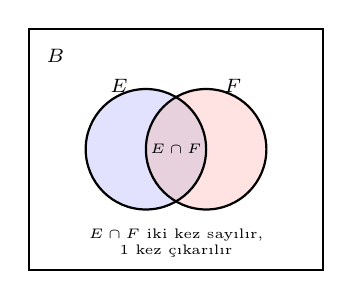
\begin{tikzpicture}[scale=0.85]

                % --- Koşul uzayı / evren (B) ---
                \draw[thick] (-2.2,-1.8) rectangle (2.2,1.8);
                \node at (-1.8,1.4) {\scriptsize $B$};

                % --- Olaylar: E ve F ---
                % Yarı saydam doldurma: kesişim doğal olarak koyulaşır
                \fill[blue!25, opacity=0.45] (-0.45,0) circle (0.9);
                \fill[red!25,  opacity=0.45] (0.45,0) circle (0.9);

                % --- Kesişimi ayrıca hafifçe vurgula (lens bölgesi) ---
                \begin{scope}
                    \clip (-0.45,0) circle (0.9);
                    \fill[black!20, opacity=0.25] (0.45,0) circle (0.9);
                \end{scope}

                % --- Sınırlar ---
                \draw[thick] (-0.45,0) circle (0.9);
                \draw[thick] (0.45,0) circle (0.9);

                % --- Etiketler ---
                \node at (-0.85,0.95) {\scriptsize $E$};
                \node at (0.85,0.95) {\scriptsize $F$};
                \node at (0,0) {\tiny $E \cap F$};

                % --- Açıklama ---
                \node[align=center, font=\tiny] at (0,-1.4)
                {$E \cap F$ iki kez sayılır,\\ 1 kez çıkarılır};

            \end{tikzpicture}
        \end{column}
    \end{columns}
\end{frame}

\subsection{Bağımlılık Sezgisi (Hafta 3'e Köprü)}
\begin{frame}[fragile]{Bağımlılık Sezgisi}
    Genel durumda:
    \[ P(A|B) \neq P(A) \]
    Bu eşitsizlik, $B$ olayının gerçekleşmesinin, $A$'nın olasılığını \textbf{değiştirdiği} (güncellediği) anlamına gelir. Bu durumda olaylar \textbf{bağımlıdır}.

    \vspace{0.3cm}
    \begin{exampleblock}{Örnek (Zar)}
        $S=\{1..6\}$. $A=\{2\}$ (Çift gelmesi değil, 2 gelmesi). $P(A)=1/6$.
        
        $B=\{2,4,6\}$ (Çift gelmesi). $P(A|B) = 1/3$.
        
        Burada $1/3 \neq 1/6$. Çift geldiğini bilmek, 2 gelme ihtimalini artırdı.
    \end{exampleblock}

    \onslide<2->{
        Eğer $P(A|B) = P(A)$ ise, $B$ bilgisi $A$'yı etkilememiştir. Bu duruma \textbf{bağımsızlık} denir (Detaylar sonraki bölümde).
    }
\end{frame}

\subsection{Pekiştirme Soruları (Sıra Sizde)}

\begin{frame}{Soru 3: Öğrenci Anketi (Kesişim ve Tümleyen)}
    Bir üniversite sınıfındaki 500 öğrenci üzerinde yapılan ankette:
    \begin{itemize}
        \item 210 öğrenci sigara içiyor ($S$),
        \item 258 öğrenci alkol kullanıyor ($A$),
        \item 122 öğrenci hem sigara hem alkol kullanıyor ($S \cap A$).
    \end{itemize}
    
    \vspace{0.2cm}
    \textbf{Sorular:}
    \begin{enumerate}
        \item[(a)] Alkol kullanan bir öğrencinin, sigara da içiyor olma olasılığı nedir? ($P(S|A)$)
        \item[(b)] Sigara içmeyen bir öğrencinin, alkol kullanıyor olma olasılığı nedir? ($P(A|S')$)
    \end{enumerate}
    
    \vspace{0.1cm}
    \textit{(İpucu: (b) şıkkı için $S'$ kümesinin büyüklüğünü ve $A \cap S'$ kesişimini düşününüz.)}
\end{frame}

\begin{frame}{Soru 3: Çözüm}
    \vspace{5cm} 
\end{frame}

\begin{frame}[allowframebreaks]{Soru 3: Detaylı Çözüm}
    \scriptsize
    {\color{red}
    \textbf{Verilen sayılar:}
    \[
    |S|=210,\quad |A|=258,\quad |S\cap A|=122,\quad |Evrensel|=500
    \]
    
    \vspace{0.1cm}
    \textbf{(a) $P(S|A)$ hesabı}
    \[
    P(S|A)=\frac{P(S\cap A)}{P(A)}=\frac{122/500}{258/500}=\frac{122}{258}
    \]
    \[
    P(S|A)\approx 0.473
    \]
    \[
    \boxed{P(S|A)\approx \%47.3}
    \]
    
    \framebreak
    \textbf{(b) $P(A|S')$ hesabı}
    
    Önce sigara içmeyenleri bulalım:
    \[
    |S'|=500-210=290
    \]
    Alkol kullanıp sigara içmeyenler:
    \[
    |A\cap S'|=|A|-|A\cap S|=258-122=136
    \]
    Şimdi koşullu olasılık:
    \[
    P(A|S')=\frac{P(A\cap S')}{P(S')}=\frac{136/500}{290/500}=\frac{136}{290}
    \]
    \[
    P(A|S')\approx 0.469
    \]
    \[
    \boxed{P(A|S')\approx \%46.9}
    \]
    }
\end{frame}

\begin{frame}{Soru 4: Elektronik Bileşen Testi (Ayrık Olaylar)}
    Bir elektronik bileşenin arızalı olabileceğini öngören test sonuçları aşağıdaki gibidir:
    \begin{itemize}
        \item Testi geçemeyip arızalanma olasılığı ($A$): $0.20$
        \item Testte arızalı çıkmasına rağmen arızalı olmayıp yıpranmış olma olasılığı ($Y$): $0.35$
        \item Testte arızalı çıkmasına rağmen sorunsuz çalışma olasılığı: $0.45$
    \end{itemize}
    (Not: Arıza ($A$) ve Yıpranma ($Y$) aynı anda olamaz, ayrıktır.)
    
    \vspace{0.3cm}
    \textbf{Sorular:}
    \begin{enumerate}
        \item[(a)] Bileşenin \textbf{arızalanmadığı} ($A'$) bilindiğine göre, yıpranma belirtisi göstermiş olma olasılığı nedir?
        \item[(b)] Bileşende \textbf{bir sorun} (arıza veya yıpranma) olduğu bilindiğine göre, bunun \textbf{arıza} kaynaklı olma olasılığı nedir?
    \end{enumerate}
\end{frame}

\begin{frame}{Soru 4: Çözüm}
    \vspace{5cm} 
\end{frame}

\begin{frame}[allowframebreaks]{Soru 4: Detaylı Çözüm}
    \scriptsize
    {\color{red}
    \textbf{Verilenler:}
    \[
    P(A)=0.20,\quad P(Y)=0.35,\quad P(\text{Sorunsuz})=0.45
    \]
    Arıza ($A$) ve yıpranma ($Y$) ayrık olduğundan $A\cap Y=\varnothing$.
    
    \vspace{0.1cm}
    \textbf{(a) $P(Y|A')$ hesabı}
    
    Önce $P(A')$:
    \[
    P(A')=1-P(A)=1-0.20=0.80
    \]
    Yıpranma, arıza olmayan durumun içindedir ($Y\subseteq A'$), bu yüzden:
    \[
    P(Y\cap A')=P(Y)=0.35
    \]
    \[
    P(Y|A')=\frac{P(Y\cap A')}{P(A')}=\frac{0.35}{0.80}=0.4375
    \]
    \[
    \boxed{P(Y|A')=0.4375=\%43.75}
    \]
    
    \framebreak
    \textbf{(b) $P(A|A\cup Y)$ hesabı}
    
    ``Bir sorun var'' olayı $A\cup Y$'dir:
    \[
    P(A\cup Y)=P(A)+P(Y)=0.20+0.35=0.55
    \]
    \[
    P(A|A\cup Y)=\frac{P(A\cap (A\cup Y))}{P(A\cup Y)}=\frac{P(A)}{0.55}=\frac{0.20}{0.55}
    \]
    \[
    P(A|A\cup Y)\approx 0.3636
    \]
    \[
    \boxed{P(A|A\cup Y)\approx \%36.36}
    \]
    }
\end{frame}

\section{Çarpım (Product/Multiplicative) Kuralı}
\subsection{İki Olay İçin Çarpım Kuralı}

\begin{frame}[fragile]{Çarpım Kuralı (Product Rule)}
    \begin{block}{Teorem 2.10}
        $P(B) > 0$ olmak üzere, $A$ ve $B$ olayları için:
        \[ P(A \cap B) = P(B) \cdot P(A|B) \]
    \end{block}

    \begin{itemize}
        \item Bu formül, koşullu olasılık tanımından ($P(A|B) = P(A \cap B)/P(B)$) içler dışlar çarpımı ile elde edilir.
        \item \textbf{Yorum:} İki olayın aynı anda (veya peş peşe) gerçekleşmesi, birincinin gerçekleşmesi VE o gerçekleştikten sonra ikincinin gerçekleşmesi demektir.
    \end{itemize}
\end{frame}

\begin{frame}[fragile]{Simetri Özelliği}
    Kesişim işlemi değişmeli olduğu için ($A \cap B = B \cap A$), sıra fark etmez:

    \[ P(A \cap B) = P(B) \cdot P(A|B) = P(A) \cdot P(B|A) \]

    \begin{alertblock}{Sonuç}
        Aynı kesişim olasılığı, olayların yazım sırası değişse de değişmez; önemli olan
        koşulun hangi olay olduğunun açıkça belirtilmesidir.
    \end{alertblock}
\end{frame}

\begin{frame}[fragile]{``Sırayla Gerçekleşme'' Yorumu}
    Çarpım kuralı, \textbf{ardışık tanımlanmış} olayların olduğu deneylerde (ör. \textbf{sampling without replacement}, yerine koymadan çekim) özellikle kullanışlıdır.

    \textbf{Örnek (Sigorta Kutusu):}
    Kutuda 20 sigorta var, 5'i bozuk. Yerine koymadan 2 sigorta çekiliyor. İkisinin de bozuk olma olasılığı?
    
    \begin{columns}[T]
        \begin{column}{0.55\textwidth}
            \centering
            \begin{tikzpicture}[
                level 1/.style={sibling distance=2.5cm, level distance=1.8cm},
                level 2/.style={sibling distance=1.5cm, level distance=1.8cm},
                edge from parent/.style={draw, -{Stealth}, thick},
                every node/.style={font=\tiny},
                label_node/.style={midway, fill=white, inner sep=1pt, font=\tiny}
            ]
            \node[circle, draw, fill=blue!20] {Başla}
                child {
                    node[circle, draw, fill=red!20, align=center] {1. Bozuk\\(B)}
                    edge from parent node[label_node] {5/20}
                    child {
                        node[circle, draw, fill=red!40, align=center] {2. Bozuk\\(B)}
                        edge from parent node[label_node] {4/19}
                    }
                    child {
                        node[circle, draw, fill=green!20, align=center] {2. İyi\\(İ)}
                        edge from parent node[label_node] {15/19}
                    }
                }
                child {
                    node[circle, draw, fill=green!20, align=center] {1. İyi\\(İ)}
                    edge from parent node[label_node] {15/20}
                    child {
                        node[circle, draw, fill=red!20, align=center] {2. Bozuk\\(B)}
                        edge from parent node[label_node] {5/19}
                    }
                    child {
                        node[circle, draw, fill=green!40, align=center] {2. İyi\\(İ)}
                        edge from parent node[label_node] {14/19}
                    }
                };
            \end{tikzpicture}
        \end{column}
        
        \begin{column}{0.43\textwidth}
            \scriptsize
            \textbf{Hesaplama:}
            \begin{itemize}
                \item $B$: Birinci bozuk. 
                \\ $P(B) = 5/20 = 1/4$
                
                \item $A$: İkinci bozuk. 
                \\ (Kalan: 4 bozuk, 19 toplam)
                
                \item $P(A|B) = 4/19$
                
                \item $P(A \cap B) = \frac{1}{4} \cdot \frac{4}{19} = \boxed{\frac{1}{19}}$
            \end{itemize}
            
            \vspace{0.2cm}
            \textbf{Yorum:} Her aşamada payda (toplam sayı) azalır!
        \end{column}
    \end{columns}
\end{frame}

\subsection{Çoklu Olaylara Genişletme (Chain Rule)}

\begin{frame}[fragile]{Zincir Kuralı (Chain Rule)}
    \begin{block}{Teorem 2.12: Genel Çarpım Kuralı}
        $k$ olay için bileşik olasılık, koşullu olasılıkların çarpımıdır:
        \[ P(A_1 \cap A_2 \cap \dots \cap A_k) = P(A_1) P(A_2|A_1) P(A_3|A_1 \cap A_2) \dots \]
    \end{block}
    
    \begin{exampleblock}{Örnek Problem: 3 Kart Çekme}
        \small
        \textbf{Soru:} 52 kartlık bir desteden \textbf{yerine koymadan} sırasıyla 3 kart çekiliyor.
        1. kartın \textbf{Kırmızı As}, 2. kartın \textbf{10 veya Vale}, 3. kartın \textbf{3--7 arası (3 ve 7 dahil)} gelme olasılığı nedir?
    \end{exampleblock}

    \onslide<2->{
        \small
        \textbf{Çözüm:}
        \begin{itemize}
            \item<2-> \textbf{Adım 1 ($A_1$):} 2 Kırmızı As var, toplam 52 kart. $\rightarrow 2/52$
            \item<3-> \textbf{Adım 2 ($A_2|A_1$):} 8 tane (10 veya Vale) var, kalan 51 kart. $\rightarrow 8/51$
            \item<4-> \textbf{Adım 3 ($A_3|A_1 \cap A_2$):} 20 tane (3--7 arası (3 ve 7 dahil)) var, kalan 50 kart. $\rightarrow 20/50$
            \item<5-> \textbf{Sonuç:} $\frac{2}{52} \cdot \frac{8}{51} \cdot \frac{20}{50} \approx 0.0024$
        \end{itemize}
    }
\end{frame}

\begin{frame}[fragile]{Uygulama Şablonu}
    \begin{columns}[T]
        \begin{column}{0.55\textwidth}
            \centering
            \begin{tikzpicture}[
                every node/.style={font=\tiny, align=center},
                arrow/.style={draw, -{Stealth}, thick}
            ]
            % Nodes (Strictly Vertical Alignment)
            \node[circle, draw, fill=orange!30, minimum size=0.8cm] (start) at (0,0) {Başla};
            \node[rectangle, draw, fill=blue!20, minimum width=1.0cm] (step1) at (0, -1.1) {$A_1$\\olur};
            \node[rectangle, draw, fill=green!20, minimum width=1.0cm] (step2) at (0, -2.2) {$A_2$\\olur};
            \node[rectangle, draw, fill=red!20, minimum width=1.0cm] (step3) at (0, -3.3) {$A_3$\\olur};
            
            % Arrows with Labels (Shifted to the side to avoid overlap)
            \draw[arrow] (start) -- node[midway, right, xshift=0.3cm] {$P(A_1)$} (step1);
            \draw[arrow] (step1) -- node[midway, right, xshift=0.3cm] {$P(A_2|A_1)$} (step2);
            \draw[arrow] (step2) -- node[midway, right, xshift=0.3cm] {$P(A_3|A_1 \cap A_2)$} (step3);
            
            % Goal Statement
            \node[below, align=center, font=\scriptsize] at (0, -4.0) {
                \textbf{Hedef:} $P(A_1 \cap A_2 \cap A_3)$ \\
                $= P(A_1) \cdot P(A_2|A_1) \cdot P(A_3|A_1 \cap A_2)$
            };
            \end{tikzpicture}
        \end{column}
        
        \begin{column}{0.43\textwidth}
            \small
            Daima olayları \textbf{kronolojik} veya \textbf{mantıksal} bir sıraya koyarak düşünün:
            
            \vspace{0.3cm}
            \begin{enumerate}
                \item \textbf{İlk olay:} Saf (koşulsuz) olasılık.
                \\ $P(A_1)$
                
                \item \textbf{İkinci olay:} Birinci gerçekleşmiş gibi düşün.
                \\ $P(A_2|A_1)$
                
                \item \textbf{Üçüncü olay:} İlk ikisi gerçekleşmiş gibi düşün.
                \\ $P(A_3|A_1 \cap A_2)$
            \end{enumerate}
            
            \vspace{0.3cm}
            Bu yöntem, karmaşık ``kesişim'' problemlerini, adım adım basit koşullu olasılıklara böler.
        \end{column}
    \end{columns}
\end{frame}

\subsection{Pekiştirme Soruları (Sıra Sizde)}

\begin{frame}{Soru 5: Serum Üretimi (Ardışık Muayene)}
    Bir grip aşısı üreticisi, ürettiği serum partilerini kalite kontrol için sırasıyla üç farklı departmandan geçiriyor. Departmanların \textbf{reddetme} (reject) oranları sırasıyla:
    \begin{itemize}
        \item 1. Departman: $0.10$
        \item 2. Departman: $0.08$
        \item 3. Departman: $0.12$
    \end{itemize}
    Denetimlerin \textbf{sıralı ve bağımsız} olduğunu varsayınız.
    
    \vspace{0.2cm}
    \textbf{Sorular:}
    \begin{enumerate}
        \item[(a)] Bir serum partisinin 1. departmanı geçip, 2. departman tarafından reddedilme olasılığı nedir?
        \item[(b)] Bir serum partisinin 1. ve 2. departmanı geçip, 3. departman tarafından reddedilme olasılığı nedir?
    \end{enumerate}
\end{frame}

\begin{frame}{Soru 5: Çözüm}
    \vspace{5cm} 
\end{frame}

\begin{frame}[allowframebreaks]{Soru 5: Detaylı Çözüm}
    \scriptsize
    {\color{red}
    \textbf{Verilen reddetme oranları:}
    \[
    r_1=0.10,\quad r_2=0.08,\quad r_3=0.12
    \]
    Geçme oranları:
    \[
    p_1=1-r_1=0.90,\quad p_2=1-r_2=0.92
    \]
    
    \vspace{0.1cm}
    \textbf{(a) 1. departmanı geçip 2.'de reddedilme}
    \[
    P(\text{Geç}_1 \cap \text{Red}_2)=P(\text{Geç}_1)\cdot P(\text{Red}_2|\text{Geç}_1)
    \]
    Bağımsızlık nedeniyle $P(\text{Red}_2|\text{Geç}_1)=P(\text{Red}_2)=0.08$:
    \[
    P=0.90\times 0.08=0.072
    \]
    \[
    \boxed{0.072=\%7.2}
    \]
    
    \vspace{0.1cm}
    \textbf{(b) 1. ve 2.'yi geçip 3.'te reddedilme}
    \[
    P(\text{Geç}_1 \cap \text{Geç}_2 \cap \text{Red}_3)=0.90\times 0.92\times 0.12
    \]
    \[
    P=0.09936
    \]
    \[
    \boxed{0.09936=\%9.936}
    \]
    
    \vspace{0.1cm}
    \textbf{Yorum:} Ardışık süreçlerde olasılık, adımların çarpımıyla bulunur (zincir/çarpım kuralı).
    }
\end{frame}

\begin{frame}{Soru 6: Elektrik Devresi (Paralel ve Seri Bağlantı)}
    Aşağıdaki gibi bir sistem düşünün:
    \begin{itemize}
        \item $A$ ve $B$ bileşenleri \textbf{seri} bağlıdır (İkisi de çalışmalı).
        \item $C$ ve $D$ bileşenleri birbirine \textbf{paralel} bağlıdır (En az biri çalışmalı).
        \item Bu iki alt sistem (AB grubu ve CD grubu) birbirine \textbf{seri} bağlıdır.
    \end{itemize}
    
    Bileşenlerin çalışma olasılıkları: $P(A)=0.9$, $P(B)=0.9$, $P(C)=0.8$, $P(D)=0.8$. Bileşenler birbirinden \textbf{bağımsız} çalışmaktadır.
    
    \textbf{Olay tanımı:} $A$: ``A bileşeni çalışır'', $B$: ``B bileşeni çalışır'', $C$: ``C bileşeni çalışır'', $D$: ``D bileşeni çalışır''.
    Bu nedenle AB seri alt sisteminin çalışması olayı $A \cap B$ ile gösterilir.
    
    \vspace{0.2cm}
    \textbf{Soru:} Tüm sistemin sorunsuz çalışma olasılığı nedir?
    
    \textit{(İpucu: Önce paralel kısmın ($C \cup D$) çalışma olasılığını bulunuz.)}
\end{frame}

\begin{frame}{Soru 6: Kritik Fikir -- $P(C\cup D)$ Neden Tamamlayıcıdan?}
    \small
    \textbf{Paralel alt sistem hedefi:} ``$C$ veya $D$ çalışsın'' $\Rightarrow$ ``en az biri çalışsın''.
    
    \vspace{0.1cm}
    Bu olay doğrudan toplanmaktan çok, değili üzerinden daha temiz bulunur:
    \[
    P(C\cup D)=1-P((C\cup D)')=1-P(C'\cap D')
    \]
    çünkü \textbf{De Morgan} kuralına göre ``en az biri çalışsın'' olayının değili ``ikisi de çalışmasın''dır.
    
    \vspace{0.1cm}
    \textbf{Kısa örnek (bu sorunun verisi):}
    \[
    P(C')=1-0.8=0.2,\qquad P(D')=1-0.8=0.2
    \]
    Bağımsızlık nedeniyle:
    \[
    P(C'\cap D')=P(C')P(D')=0.2\times 0.2=0.04
    \]
    \[
    \Rightarrow\ P(C\cup D)=1-0.04=0.96
    \]
\end{frame}

\begin{frame}[allowframebreaks]{Soru 6: Detaylı Çözüm}
    \scriptsize
    {\color{red}
    \textbf{Sistem yapısı:} $(A\text{-}B)$ seride, $(C\text{-}D)$ paralelde; sonra bu iki grup kendi aralarında seri.
    
    \vspace{0.1cm}
    \textbf{Adım 1 -- AB seri alt sistemi}
    Burada $A \cap B$, ``A ve B birlikte çalışır'' olayıdır (bazı kaynaklarda kısaca $AB$ de yazılır).
    \[
    P(A\cap B)=P(A)\cdot P(B)=0.9\times 0.9=0.81
    \]
    
    \vspace{0.1cm}
    \textbf{Adım 2 -- CD paralel alt sistemi}
    Paralelde en az biri çalışmalı:
    \[
    P(C\cup D)=1-P(C'\cap D')
    \]
    \[
    P(C'\cap D')=(1-0.8)(1-0.8)=0.2\times 0.2=0.04
    \]
    \[
    P(C\cup D)=1-0.04=0.96
    \]
    
    \vspace{0.1cm}
    \textbf{Adım 3 -- İki alt sistemi seri bağla}
    \[
    P(\text{Sistem})=P(A\cap B)\cdot P(C\cup D)=0.81\times 0.96=0.7776
    \]
    
    \vspace{0.1cm}
    \textbf{Sonuç:}
    \[
    \boxed{P(\text{Sistem sorunsuz})=0.7776=\%77.76}
    \]
    }
\end{frame}

\section{Hafta 2 Kapanış}
\subsection{Özet ve Alıştırma Tipleri}
\begin{frame}{``Koşullu Olasılık'' Problem Tipleri}
    Koşullu olasılık problemleri genellikle üç ana yöntemle çözülür:

    \begin{enumerate}
        \item \textbf{Tablo Yöntemi:} Veriler iki boyutlu (kontenjans) tablo halindeyse.
        \begin{itemize}
            \item Satır/sütun toplamları üzerinden doğrudan oranlanır.
            \item Örnek: Kadın/Erkek çalışan tablosu.
        \end{itemize}
        
        \item \textbf{Ağaç Diyagramı (Tree Diagram):} Olaylar sıralı/ardışık gerçekleşiyorsa.
        \begin{itemize}
            \item Dallar üzerinde koşullu olasılıklar ($P(A|B)$), yol sonlarında kesişim olasılıkları ($P(A \cap B)$) bulunur.
            \item Örnek: Kusurlu ürün testi, ardışık kart çekimi.
        \end{itemize}

        \item \textbf{Venn Diyagramı:} Kümeler ve bölgelerin büyüklükleri biliniyorsa.
        \begin{itemize}
            \item $P(A \cap B)$ ve $P(A)$ görsel olarak bellidir.
        \end{itemize}
    \end{enumerate}
\end{frame}

\begin{frame}[fragile]{Mini-Quiz: $P(A \cap B)$ mi $P(A|B)$ mi?}
    Aşağıdaki cümlelerin hangisinde hangi olasılık kastedilmektedir?
    
    \begin{itemize}[<+->]
        \item \textbf{Soru 1:} ``Rastgele seçilen bir kişinin hem gözlüklü hem de şapkalı olma olasılığı nedir?''
        \item[] \textcolor{blue}{$\Rightarrow P(\text{Gözlük} \cap \text{Şapka})$} \hspace{0.2em} \andbadge
        
        \item \textbf{Soru 2:} ``Şapkalı olduğu bilinen bir kişinin gözlüklü de olma olasılığı nedir?''
        \item[] \textcolor{red}{$\Rightarrow P(\text{Gözlük} | \text{Şapka})$} \hspace{0.2em} \givenbadge
        
        \item \textbf{Soru 3:} ``\textbf{Yerine koymadan} iki kart çekiliyor: Birincinin As ve ikincinin Papaz gelme olasılığı?''
        \item[] \textcolor{blue}{$\Rightarrow P(\text{As}_1 \cap \text{Papaz}_2)$} \hspace{0.2em} \andbadge
        
        \item \textbf{Soru 4:} ``\textbf{Yerine koymadan} ilk kart As geldi. İkincinin Papaz gelme ihtimali kaç kaldı?''
        \item[] \textcolor{red}{$\Rightarrow P(\text{Papaz}_2 | \text{As}_1)$} \hspace{0.2em} \givenbadge
    \end{itemize}
\end{frame}

\begin{frame}{Çıkış Bileti: 3 Satırda ``Koşullama''}
    Dersi bitirirken kendinize şu soruları sorun:
    
    \begin{block}{Refleksiyon}
        \begin{enumerate}
            \item ``Verildiğinde'' (given) dendiğinde örneklem uzayıma ($S$) ne olur? Küçülür mü?
            \item $P(A|B)$ ile $P(B|A)$ aynı şey midir? (Genellikle hayır!)
            \item Bağımsızlık durumunda $P(A|B)$ neye eşit olur? ($P(A)$'ya!)
        \end{enumerate}
    \end{block}
    
    \vspace{0.3cm}
    \centering
    \textit{Haftaya: Bağımsızlık (Independence), Bayes Kuralı ve Toplam Olasılık.}
\end{frame}

\section{Kaynaklar}
\begin{frame}[allowframebreaks]{Kaynaklar}
    \nocite{*}
    \printbibliography{}
\end{frame}

\section{Haftalık Uygulama}
\begin{frame}{Sıra Sizde: Kaggle Uygulaması}
    \justifying{}
    Koşullu olasılık simülasyonları için Python notebook'u hazırladık.
    
    \vspace{0.5cm}
    \begin{enumerate}
        \item \textbf{Adım 1:} \href{https://www.kaggle.com}{Kaggle.com} hesabınıza giriş yapın.
        \item \textbf{Adım 2:} Aşağıdaki linkten dersin defterine gidin:
        
        \vspace{0.3cm}
        \begin{center}
             \hrefcol{https://www.kaggle.com/code/ufukasil/mat204-olasilik-ve-stat-st-k-2-hafta}{Kaggle Notebook: Koşullu Olasılık Simülasyonu}
        \end{center}
        \vspace{0.3cm}
        
        \item \textbf{Adım 3:} \textbf{"Copy \& Edit"} butonuna basarak kendi kopyanız üzerinde çalışın.
    \end{enumerate}
\end{frame}

\section{Yapay Zeka Asistanı}
\begin{frame}{Yapay Zeka Asistanınız: NotebookLM}
    \begin{columns}[T]
        \begin{column}{0.48\textwidth}
            \justifying{}
            \textbf{Ders Materyalleri ile Etkileşime Geçin!}
            
            Bu dersin tüm içeriği (sunumlar, makaleler ve notlar), Google'ın gelişmiş yapay zeka asistanı \textbf{NotebookLM} sistemine yüklenmiştir.
            
            \vspace{1em}
            \begin{itemize}
                \item \textbf{Anında Cevaplar:} Aklınıza takılanları sorun.
                \item \textbf{Özetler:} Karmaşık konuları basitçe öğrenin.
                \item \textbf{Audio Overview:} Dersi bir podcast gibi dinleyin.
            \end{itemize}
            
            \vspace{1.5em}
            \begin{center}
                {\setbeamercolor{button}{bg=red,fg=black}
                \href{https://notebooklm.google.com/notebook/37796201-25fd-4d44-aa3c-b673ce22f7a4}{\beamerbutton{\rule[-4ex]{0pt}{11ex}\Large \textbf{Hemen Deneyin}}}}
            \end{center}
        \end{column}
        
        \begin{column}{0.48\textwidth}
            \centering
            \includegraphics[width=\textwidth, height=0.6\textheight, keepaspectratio]{figures/notebooklm.jpg}
        \end{column}
    \end{columns}
\end{frame}

\begin{frame}[plain,noframenumbering]
    \begin{tikzpicture}[remember picture,overlay]
        \node[anchor=center, at=(current page.center), inner sep=0pt] {
            \includegraphics[width=\paperwidth, height=\paperheight]{figures/combined_qrs.png}
        };
        \node[anchor=south, at=(current page.south), yshift=0.5cm, fill=white!95, rounded corners, inner sep=10pt, text width=0.95\paperwidth, align=center] {
            \Large \textbf{\textcolor{blue}{Bizi Takip Edin!}} \\
            \vspace{0.3em}
            \small Ders tekrarlarıyla konuları pekiştirmek (YouTube), profesyonel proje ağlarına katılmak (LinkedIn) ve kampüs duyurularından anında haberdar olmak (Instagram) için topluluğumuza katılın.
        };
    \end{tikzpicture}
\end{frame}

\end{document}
